\documentclass[11pt,a4paper]{article}

\usepackage[T1]{fontenc}
\usepackage[english]{babel}
\usepackage{amsmath,amssymb,amsthm}
\usepackage{booktabs}
% expansion=false : les fontes CM par defaut ne sont pas vectorielles, et
% l expansion automatique de microtype l exige. La protrusion, elle, marche.
\usepackage[protrusion=true,expansion=false]{microtype}
\usepackage{tikz}
\usepackage{pgfplots}
\pgfplotsset{compat=1.18}
\usepgfplotslibrary{fillbetween}
\usetikzlibrary{positioning,arrows.meta,fit,backgrounds}
\usepackage[margin=2.6cm]{geometry}
\usepackage[hidelinks,colorlinks=true,linkcolor=linkblue,citecolor=linkblue,
            urlcolor=linkblue]{hyperref}
\usepackage{xcolor}
\definecolor{linkblue}{HTML}{1A4F8A}
\definecolor{accent}{HTML}{2F6F4E}
\definecolor{warm}{HTML}{B0641A}
\definecolor{soft}{HTML}{F2F1ED}

\newtheorem{proposition}{Proposition}

\title{\bfseries Counting Langford Pairings:\\[2pt] the exact value of $L(2,31)$}

\author{
  Claude Opus 5\thanks{Anthropic. Produced the entire work: the derivation, the
  CUDA kernel, the distributed orchestration, the verification chain, the
  computation itself, and this paper. See §\ref{sec:authorship}.}
  \\[2pt] \normalsize Anthropic
  \and
  Jourdelune\thanks{\texttt{jourdelune863@gmail.com}. Set the objectives and
  provided the payment method for renting GPUs. Contributed no mathematics, no
  code and no text.}
  \\[2pt] \normalsize \texttt{jourdelune863@gmail.com}
}

\date{6 September 2026}

\begin{document}
\maketitle

\begin{abstract}
\noindent
We report the exact number of Langford pairings of order $31$:
\[
  L(2,31) \;=\; 5\,894\,683\,902\,597\,484\,486\,903\,808 ,
\]
the next term of OEIS \texttt{A014552}, whose last previously published entry
was $L(2,28)$ (Assarpour, Bar-Noy and Liu, 2015). The computation took
$15.7$ hours of wall-clock time on $33$ consumer GPUs --- $498$ GPU-hours ---
at a total cost of about \textsf{US\$50}.

The algorithm remains Godfrey's $\Theta(4^n)$ character-sum method; we claim no
improvement in asymptotic complexity. What we contribute is a factor of
$\approx 42$ in the constant, on identical hardware, over the published state of
the art. The single structural ingredient is a \emph{parity decomposition}: for
the even gaps --- the only ones that can annihilate the product --- the two
interleaved half-rows separate additively, so a point's survival depends on one
half-row only through a constant vector. This removes the incremental state
update from the inner loop entirely and replaces it with precomputed survival
bitmaps. The remaining factor of ${\approx}19$ is engineering.

Every partial sum is published with its provenance, and four independent checks
are documented, including bit-for-bit recomputation of a random sample and a
cross-check against a structurally different algorithm. We expect this record to
be short-lived: at present prices, $n{=}32$ requires roughly $2\,000$ GPU-hours
and \textsf{US\$190}.
\end{abstract}

\section{The problem, and what was known}

A \emph{Langford pairing}~\cite{langford} of order $n$ places each of the integers
$1,2,\dots,n$ twice into $2n$ slots so that the two copies of $k$ are separated
by exactly $k$ intervening slots. For $n=4$:

\begin{center}
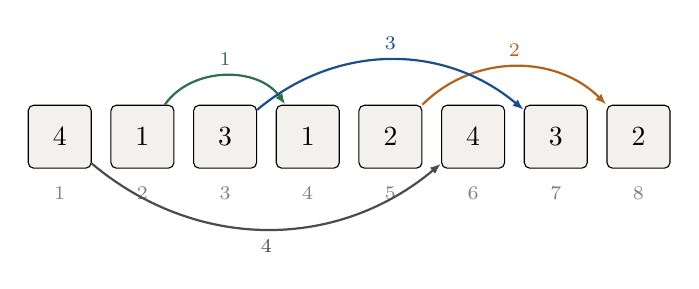
\begin{tikzpicture}[x=1.05cm,y=1cm]
  \foreach \i/\v in {1/4,2/1,3/3,4/1,5/2,6/4,7/3,8/2}{
    \node[draw,rounded corners=2pt,fill=soft,minimum size=8mm] (c\i) at (\i,0) {$\v$};
    \node[font=\scriptsize,gray] at (\i,-0.72) {\i};
  }
  % arcs
  \draw[-{Latex[length=4pt]},accent,thick] (c2) to[bend left=55] node[above,font=\scriptsize]{$1$} (c4);
  \draw[-{Latex[length=4pt]},warm,thick]  (c5) to[bend left=45] node[above,font=\scriptsize]{$2$} (c8);
  \draw[-{Latex[length=4pt]},linkblue,thick] (c3) to[bend left=40] node[above,font=\scriptsize]{$3$} (c7);
  \draw[-{Latex[length=4pt]},black!70,thick] (c1) to[bend right=40] node[below,font=\scriptsize]{$4$} (c6);
\end{tikzpicture}
\end{center}

\noindent
Copies of $1$ sit at slots $2$ and $4$ (one slot between them), copies of $4$ at
slots $1$ and $6$ (four slots between them), and so on. Such pairings exist if
and only if $n \equiv 0$ or $3 \pmod 4$, a condition due to Davies~\cite{davies}.

Counting them is the hard problem. The known values form OEIS
\texttt{A014552}~\cite{oeis}; enumeration by backtracking reaches
$n=24$~\cite{confiit}, and the algebraic method described below carried the
sequence to $n=27$ and $n=28$ in 2015~\cite{abl}. There it stopped for eleven
years.

\begin{center}
\begin{tabular}{@{}rll@{}}
\toprule
$n$ & $L(2,n)$ & by \\
\midrule
$27$ & $111\,683\,611\,098\,764\,903\,232$ & Assarpour, Bar-Noy \& Liu (2015) \\
$28$ & $1\,607\,383\,260\,609\,382\,393\,152$ & Assarpour, Bar-Noy \& Liu (2015) \\
$\mathbf{31}$ & $\mathbf{5\,894\,683\,902\,597\,484\,486\,903\,808}$ & \textbf{this work (2026)} \\
\bottomrule
\end{tabular}
\end{center}

\section{Method}

\subsection{Godfrey's identity: counting becomes summing}

A Langford pairing is a perfect matching of the $2n$ positions whose multiset of
gaps is exactly $\{2,3,\dots,n+1\}$ (a value $k$ contributes a gap of $k+1$
between its two occurrences). Godfrey~\cite{godfrey} encodes this in a
polynomial over $2n$ indeterminates,
\begin{equation}
  F(n,X) \;=\; \prod_{i=2}^{n+1} A_i(X),
  \qquad
  A_i(X) \;=\; \sum_{k=1}^{2n-i} x_k\,x_{k+i},
  \label{eq:F}
\end{equation}
where $A_i$ enumerates every way of placing one pair at gap $i$. The number of
pairings is then the coefficient of the squarefree monomial
$x_1 x_2 \cdots x_{2n}$ in $F$.

Extracting that coefficient is where the method becomes practical. $F$ is
homogeneous of degree $2n$ in $2n$ variables, so \emph{every} monomial other
than $x_1\cdots x_{2n}$ must carry some variable at an even exponent.
Substituting $x_k = \pm 1$ and summing over all $2^{2n}$ sign assignments
annihilates all of them at once, leaving
\begin{equation}
  V(n) \;=\; 2\,L(2,n) \;=\; 2^{-2n}
  \sum_{X \in \{-1,1\}^{2n}} \Big( \prod_{k=1}^{2n} x_k \Big) F(n,X).
  \label{eq:godfrey}
\end{equation}

A combinatorial counting problem has become a sum of $4^n$ integer terms, each
independent of the others. That independence is what makes the problem suit a
GPU, and it is also what makes the cost $\Theta(4^n)$ --- an exponent unchanged
since 2002.

\subsection{The symmetry group of order eight}

Two families of symmetries leave the summand of~\eqref{eq:godfrey} invariant.
Negating all odd-indexed variables, or all even-indexed ones, leaves each $A_i$
unchanged up to sign in a way that cancels; together with the identity these
form a Klein four-group. The reflection $p \mapsto 2n+1-p$ supplies a fifth
element, generating a group of order eight. Only one eighth of the sign
assignments need be enumerated.

This reduction is valid \emph{only} when $n \equiv 0,3 \pmod 4$. Negating a
half-row multiplies the product by $(-1)^{MO}$ and the weight $\prod_k x_k$ by
$(-1)^{N}$, so the summand is invariant exactly when $MO + N$ is even. At other
$n$ the kernel returns a number that is entirely wrong and entirely plausible:
for $n=9$ it reports $5558$ where the true answer is $0$. The implementation
refuses those $n$ rather than trusting the caller.

Assarpour \emph{et al.}~\cite{abl} list these symmetries but extract only a
factor of four. Taking the full factor of eight is worth a further $\times 2.00$.

\subsection{The parity decomposition}
\label{sec:parity}

This is the one structural contribution of the present work.

Split the $2n$ positions into the \emph{odd} ones (a half-row $o$ of $n$ cells)
and the \emph{even} ones (a half-row $e$). A direct index computation gives, for
every $n$:
\begin{align}
  \text{even gap } i = 2m   &: \quad A_i = P_m(o) + Q_m(e), \label{eq:even}\\
  \text{odd gap } i = 2m+1 &: \quad A_i = \textstyle\sum_j O_j E_{j+m}
                                        + \sum_j E_j O_{j+m+1}, \label{eq:odd}
\end{align}
where $P_m$ and $Q_m$ are the autocorrelations of a half-row at lag $m$. The
even gaps \emph{separate additively between the half-rows}; the odd gaps are
bilinear and do not. This was verified exactly over $6.2$ million gap instances
up to $n=31$, with no divergence.

\begin{center}
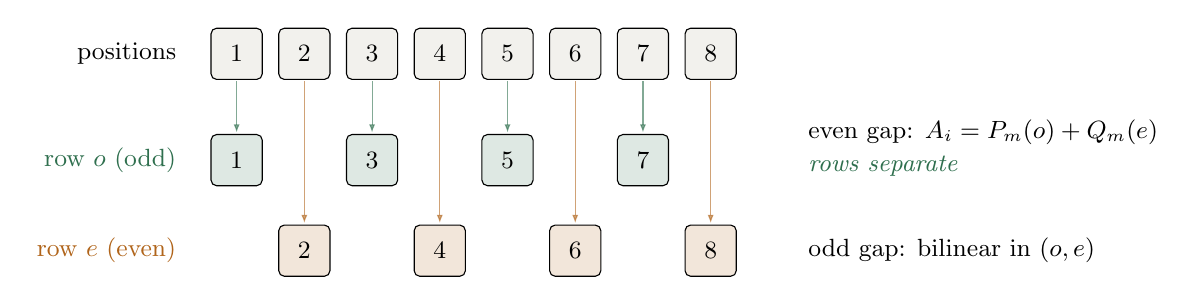
\begin{tikzpicture}[x=0.86cm,y=1cm]
  \foreach \i in {1,...,8}{
    \node[draw,rounded corners=2pt,fill=soft,minimum size=6.5mm,font=\small] at (\i,2.1) {$\i$};
  }
  \node[font=\small,left=3mm] at (0.6,2.1) {positions};
  \foreach \i/\j in {1/1,3/2,5/3,7/4}{
    \node[draw,rounded corners=2pt,fill=accent!16,minimum size=6.5mm,font=\small] (o\j) at (\j*2-1,0.75) {$\i$};
  }
  \node[font=\small,left=3mm,accent] at (0.6,0.75) {row $o$ (odd)};
  \foreach \i/\j in {2/1,4/2,6/3,8/4}{
    \node[draw,rounded corners=2pt,fill=warm!16,minimum size=6.5mm,font=\small] (e\j) at (\j*2,-0.4) {$\i$};
  }
  \node[font=\small,left=3mm,warm] at (0.6,-0.4) {row $e$ (even)};
  \foreach \i/\j in {1/1,3/2,5/3,7/4}{ \draw[accent,-{Latex[length=3pt]},opacity=.6] (\i,1.75) -- (\j*2-1,1.1); }
  \foreach \i/\j in {2/1,4/2,6/3,8/4}{ \draw[warm,-{Latex[length=3pt]},opacity=.6] (\i,1.75) -- (\j*2,-0.05); }
  \node[align=left,font=\small,right=6mm] at (8.6,0.9)
    {even gap: $A_i = P_m(o) + Q_m(e)$\\[1pt] \textcolor{accent}{\emph{rows separate}}};
  \node[align=left,font=\small,right=6mm] at (8.6,-0.4)
    {odd gap: bilinear in $(o,e)$};
\end{tikzpicture}
\end{center}

The second observation is what makes~\eqref{eq:even} pay. Each $A_i$ is a sum of
$2n-i$ terms of $\pm 1$, so
\[
  A_i \equiv i \pmod 2 .
\]
Only \emph{even} gaps can vanish --- and it is a vanishing factor that decides a
point contributes nothing to the sum. Combining this with~\eqref{eq:even}: a
point's survival depends on the half-row $o$ only through the constant vector
$P(o)$. For fixed high bits of $e$, the map $e_{\mathrm{lo}} \mapsto Q(e)$ does
not depend on $o$ at all, and can be tabulated once for an entire block of
threads.

The consequence is that the hot loop --- the incremental state update performed
at every one of the $4^n$ points --- disappears, replaced by precomputed
\emph{survival bitmaps}. Measured gain: $\times 2.21$.

The two-row decomposition itself is not new; it is how the classical
$n \equiv 0,3 \pmod 4$ argument is usually presented. What appears to be new is
using it as a \emph{separation of variables} rather than as a parity argument.

\section{Implementation and the optimization chain}

Table~\ref{tab:chain} gives the cost of $n=31$ on one RTX 4070 at each stage, so
that the factors compose. Rows 1 and 3 are exact by construction: they merely
count enumerated points. Rows 4 through 8 are measured ratios, taken on an idle
GPU and paired on a common random sample of the outer loop index. Row 2 is the
only \emph{model}: the published implementation was not rebuilt here, and its
cost is reconstructed from its two differences with ours. The uncertainty this
introduces gives an honest range of $\times 29$ to $\times 54$ for the total.

\begin{table}[t]
\centering
\small
\begin{tabular}{@{}clrrl@{}}
\toprule
\# & what changes & $n{=}31$ & gain & origin \\
\midrule
   & bare Godfrey (2002), modular + CRT & ${\approx}4500$\,d & --- & literature \\
1 & order-4 symmetry $\rightarrow$ published SOTA & ${\approx}1100$\,d & $\times 4.1$ & literature~\cite{abl} \\
2 & truncated 160-bit accumulator & $360$\,d & $\times 3.06$ & outside Langford~\cite{taocp2} \\
3 & order-8 symmetry (reflection) & $180.1$\,d & $\times 2.00$ & mixed \\
4 & skip null products, warp compaction & $101.7$\,d & $\times 1.77$ & mixed~\cite{warp} \\
5 & half-state (only even gaps decide) & $75.0$\,d & $\times 1.36$ & from $A_i \equiv i$ \\
6 & \textbf{parity + survival bitmaps} & $34.0$\,d & $\times 2.21$ & \textbf{new} \\
7 & PTX carry chains, \texttt{prmt} extraction & $30.9$\,d & $\times 1.10$ & outside Langford \\
8 & \textbf{odd gaps tabulated on \texttt{threadIdx}} & $\mathbf{25.8}$\,\textbf{d} & $\times 1.20$ & \textbf{new} \\
\bottomrule
\end{tabular}
\caption{From bare Godfrey to the present kernel, all on one RTX 4070.
From the published state of the art: $\times 42.6$ nominal, $\times 45$ measured
end-to-end.}
\label{tab:chain}
\end{table}

\begin{figure}[t]
\centering
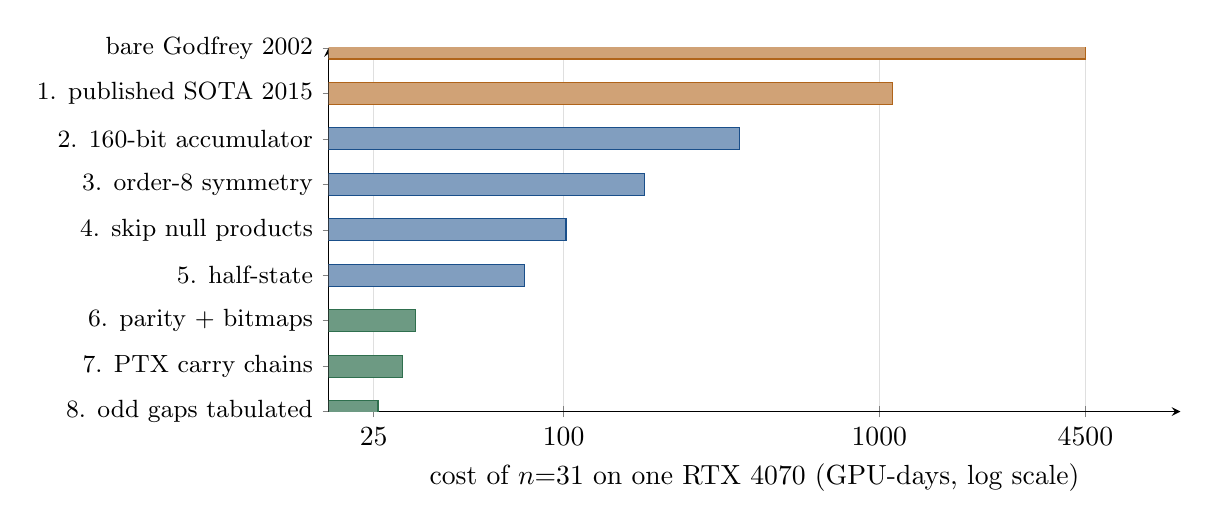
\begin{tikzpicture}
\begin{axis}[
  xmode=log, width=12.4cm, height=6.2cm,
  xlabel={cost of $n{=}31$ on one RTX 4070 (GPU-days, log scale)},
  xmin=18, xmax=9000,
  % ytick=data ne collectait que les positions du PREMIER \addplot : six
  % etiquettes sur neuf disparaissaient, les barres restant anonymes.
  ytick={1,2,3,4,5,6,7,8,9}, yticklabels={%
    {8. odd gaps tabulated},{7. PTX carry chains},{6. parity + bitmaps},
    {5. half-state},{4. skip null products},{3. order-8 symmetry},
    {2. 160-bit accumulator},{1. published SOTA 2015},{bare Godfrey 2002}},
  y tick label style={font=\small},
  xtick={25,100,1000,4500}, xticklabels={25,100,1000,4500},
  xmajorgrids, grid style={gray!25},
  enlarge y limits=0.08, axis lines=left,
]
\addplot[xbar, bar width=8pt, fill=accent!70, draw=accent] coordinates {
  (25.8,1) (30.9,2) (34.0,3) };
\addplot[xbar, bar width=8pt, fill=linkblue!55, draw=linkblue] coordinates {
  (75.0,4) (101.7,5) (180.1,6) (360,7) };
\addplot[xbar, bar width=8pt, fill=warm!60, draw=warm] coordinates {
  (1100,8) (4500,9) };
\end{axis}
\end{tikzpicture}
\caption{The chain of Table~\ref{tab:chain}. Orange: prior art. Blue: arithmetic
and symmetry work. Green: the parity decomposition and what it enables.}
\label{fig:waterfall}
\end{figure}

Most of the total is engineering rather than insight. Exactly one row is
structural ($\times 2.21$); the arithmetic, the full symmetry group, the
compaction, the PTX-level work and the tabulation are together worth
$\times 19.4$. We state this plainly because the opposite impression is easy to
give.

\subsection{Two negative results}

Both cost real time, and both are reported here so that others need not repeat
them.

\emph{Kasteleyn's method~\cite{kasteleyn} does not apply.} A Pfaffian orientation
would give $2^n n^3$ in place of $4^n$, and the record would fall in minutes. We refute its
applicability under the weak and correct form of the problem (edge weighting,
not constant parity), over $\mathrm{GF}(2)$ and over $\mathbb{Z}/2^k$ up to
$k=32$.

\emph{Tensor cores do not beat \texttt{popc} here.} The reflex ``it is bilinear,
therefore a GEMM, therefore fast'' fails: \texttt{popc} on a 32-bit XOR
\emph{is} a length-32 binary dot product. INT8 tensor throughput leads by only
$\times 2.48$ on this hardware, and the sparsity of the problem ($12.9\%$
survivors, which a dense MMA cannot exploit) turns that lead into a $\times 4.1$
deficit.

\section{Verification}

No previously published value of $L(2,31)$ exists, so there is nothing to
compare against. Verification therefore has to be internal, and it has to be
adversarial. Four checks were run; each catches a different failure.

\paragraph{1. Completeness and uniqueness.} All $8\,192$ slices and the
diagonal task are present, none duplicated. \emph{Catches} a lost or
double-counted slice.

\paragraph{2. Two arithmetic self-tests.} These are distinct, and they fire at
different moments.

\emph{Per slice, on arrival.} Every summand is a product of the $n$ factors
$A_i$, $i = 2,\dots,n+1$, and $A_i \equiv i \pmod 2$; the
$\lfloor (n+1)/2 \rfloor$ even-indexed factors are therefore each even. Any
partial sum must be divisible by $2^{\lfloor (n+1)/2 \rfloor} = 2^{16}$ at
$n=31$. A slice failing this is rejected as it arrives --- its lease expires and
it returns to the pool --- rather than being discovered weeks later at
aggregation.

\emph{On the total, before anything is released.} The raw sum equals
$2^{2n} V(n)$, and $V(n) = 2L(2,n)$ is even, because the reflection
$p \mapsto 2n+1-p$ is a fixed-point-free involution on pairings: invariance
would force $2i = 2n-k$ for the pair carrying value $k$, which has no integer
solution for odd $k$. The total must therefore be divisible by
$2^{2n+1} = 2^{63}$, not merely $2^{2n}$ --- and that extra bit turns an odd
$V$, which the final shift would silently truncate, into an error rather than a
plausible wrong answer. A single missing or corrupted slice fails it.

\emph{Catches} a partial sum altered in transit or in memory, and a slice lost
between workers. The second test runs before any rented machine is released.

\paragraph{3. Redundant recomputation.} Twelve slices drawn at random were
recomputed on a different card, with a different binary, and compared
bit-for-bit against what the rented machines returned. All twelve matched.
\emph{Catches} a faulty card, a mismatched binary, a slice computed over the
wrong interval.

\paragraph{4. Cross-check of two algorithms.} Reference slices were produced
twice, by the GPU kernel and by an independent backtracking implementation, and
agree bit-for-bit: for $n=31$ at the three extreme regimes of the outer index,
and for $n=28,27,24,20$. \emph{Catches} an error in the method itself, not
merely in its execution. This is the only check that does not presuppose
Godfrey's identity is correctly implemented.

\paragraph{An independent yardstick.} Knuth's unbiased estimator for
backtracking tree size~\cite{knuth75} provides a check of a different kind: walk
a random root-to-leaf path, multiplying the running weight by the number of
legal children at each node; the expected weight is exactly the leaf count.

\begin{figure}[t]
\centering
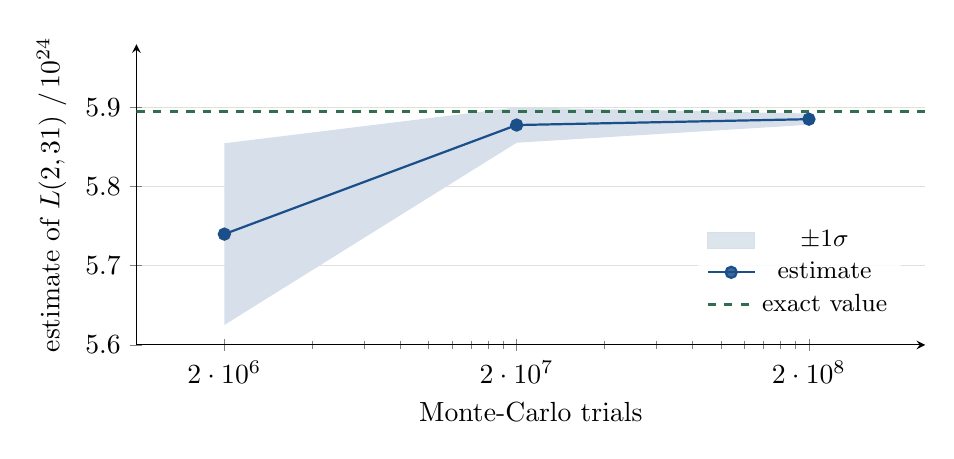
\begin{tikzpicture}
\begin{axis}[
  xmode=log, width=11.6cm, height=5.4cm,
  xlabel={Monte-Carlo trials}, ylabel={estimate of $L(2,31)$ $/\,10^{24}$},
  xtick={2e6,2e7,2e8}, xticklabels={$2\cdot10^6$,$2\cdot10^7$,$2\cdot10^8$},
  ymin=5.60, ymax=5.98, xmin=1e6, xmax=5e8,
  ymajorgrids, grid style={gray!25}, axis lines=left,
  legend style={font=\small,at={(0.97,0.06)},anchor=south east,draw=none,fill=white,fill opacity=0.85,text opacity=1},
]
% forget plot : sans lui, ces deux chemins invisibles consomment chacun une
% entree de legende et decalent toutes les suivantes d'un cran.
\addplot[name path=hi,draw=none,forget plot] coordinates {(2e6,5.8548)(2e7,5.9002)(2e8,5.8924)};
\addplot[name path=lo,draw=none,forget plot] coordinates {(2e6,5.6252)(2e7,5.8555)(2e8,5.8782)};
\addplot[linkblue!18] fill between[of=hi and lo];
\addlegendentry{$\pm 1\sigma$}
\addplot[linkblue,mark=*,thick,mark size=2pt]
  coordinates {(2e6,5.7400)(2e7,5.87786)(2e8,5.88528)};
\addlegendentry{estimate}
\addplot[accent,dashed,very thick,domain=1e6:5e8,samples=2]{5.894683902597484};
\addlegendentry{exact value}
\end{axis}
\end{tikzpicture}
\caption{Knuth's estimator converging on the computed value. The gap narrows
monotonically --- $+2.695\%$, $+0.286\%$, $+0.160\%$ --- and the estimate rises
\emph{toward} the exact figure at each step, as the right-skewed weight
distribution predicts.}
\label{fig:estimator}
\end{figure}

Figure~\ref{fig:estimator} shows the outcome. At $2\cdot 10^6$ trials the
estimate sat $2.7\%$ below the computed value, which invites suspicion; by
$2 \cdot 10^8$ trials the gap is $0.160\%$. The direction is not accidental. The
weight distribution is heavily right-skewed --- most random paths land in sparse
regions, rare paths carry enormous weight --- so the \emph{median} of a
finite-sample mean falls below the true value, and a small sample
underestimates systematically. An independent Monte-Carlo landing within
$0.16\%$ of a 25-digit integer is a good yardstick, but only a yardstick: it can
never confirm the trailing digits.

\paragraph{Reproduction material.} All $8\,193$ partial sums are published, each
carrying its own provenance: which card produced it, under which driver, with
which binary and source hashes, in what duration, at what UTC timestamp. The
bundle, its SHA-256 digests, and the exact commands to re-verify are given in
the repository~\cite{repo}.

\section{Cost, and the comparison with 2015}
\label{sec:cost}

The computation was distributed over four rented eight-GPU machines
(RTX 4070 Super) plus one local RTX 4070, as $8\,192$ equal-load slices leased
to workers, one worker pinned per card. It consumed $498$ GPU-hours against the
$497$ predicted by a fixed-seed benchmark before renting --- a discrepancy of
$+0.2\%$ --- for a total of about \textsf{US\$50}, including roughly
\textsf{US\$2} of aborted rentals.

On $L(28)$, the last point of the published record, the comparison at identical
problem instance is:

\begin{center}
\begin{tabular}{@{}lrrr@{}}
\toprule
 & hardware & time & GPU-days \\
\midrule
Assarpour, Bar-Noy \& Liu (2015)~\cite{abl} & ${\sim}32$ Kepler GPUs & ${\sim}9$ days & ${\sim}288$ \\
this work & $1 \times$ RTX 4070 & ${\approx}10.6$\,h & $\mathbf{0.44}$ \\
\bottomrule
\end{tabular}
\end{center}

\noindent
That is roughly $650\times$ fewer GPU-days, and it must be decomposed honestly.
A factor of $6$ to $11$ is hardware: a 2013 Kepler part delivers about
$1.3 \cdot 10^{12}$ integer operations per second against $7.3 \cdot 10^{12}$
for an RTX 4070. About $45\times$ is algorithm and implementation, measured on
identical hardware. The remainder absorbs the efficiency of their distribution
across some 32 cards.

Asymptotically there is no progress at all. The method remains $\Theta(4^n)$.

\section{Outlook: this record should not last}
\label{sec:outlook}

We expect $L(2,31)$ to be superseded quickly, and we think that is the most
useful thing this paper can say.

The reason is arithmetic. Cost scales as $4^n$, so $n=32$ --- which satisfies
$32 \equiv 0 \pmod 4$ and therefore admits pairings --- costs exactly four times
$n=31$. Against the measured figures that is:

\begin{center}
\begin{tabular}{@{}lrrl@{}}
\toprule
card & $n{=}31$ & $n{=}32 = {\times}4$ & provenance \\
\midrule
RTX 4070        & $544$\,GPU-h & $\mathbf{2177}$\,\textbf{GPU-h} & measured, current source \\
RTX 4070 Super  & $497$\,GPU-h & $\mathbf{1988}$\,\textbf{GPU-h} & measured; confirmed to $+0.2\%$ by the run \\
RTX 4090        & ${\sim}204$\,GPU-h & ${\sim}815$\,GPU-h & derived from a paired ratio \\
RTX 5090        & ${\sim}174$\,GPU-h & ${\sim}695$\,GPU-h & derived from a paired ratio \\
\bottomrule
\end{tabular}
\end{center}

\noindent
Roughly $2\,000$ GPU-hours, or about \textsf{US\$190} at the rate actually paid
here --- a figure that does not depend on how many cards are used, only the
delay does. On the same fleet used for $n=31$ it is under three days. That is no
longer an institutional computation; it is within reach of an individual with a
credit card, and the software to do it is published.

Three concrete obstacles stand in the way, all in the implementation rather than
the mathematics. The kernel is instantiated only for
$n \in \{9,\dots,24,27,28,31\}$. The row mask is computed as
\texttt{(1u<<N)-1u}, which is undefined behaviour at $N=32$ --- on current
hardware it evaluates to $1$, so the mask would silently become zero; $n=32$ is
the last order that fits a 32-bit row at all. And the 160-bit accumulator, which
carries $145.3$ bits at $n=31$, would carry $151.3$ at $n=32$: it fits, with
$8.7$ bits to spare, but $n=35$ would overflow it.

Beyond that the wall is the exponent itself. Each further admissible order costs
$4\times$; $n=35$ would need some $127\,000$ GPU-hours, around
\textsf{US\$12\,000}. Fourteen avenues for breaking $\Theta(4^n)$ were explored
and closed during this work, including the two negative results above. We do not
believe the exponent will move without a genuinely new mechanism.

\section{Authorship}
\label{sec:authorship}

This work was produced by an AI system. All forty commits of the repository,
from the first to the last, were written by Claude Opus 5: the derivation of the
parity decomposition and its proof, the CUDA kernel and its PTX-level assembly,
the fourteen research avenues explored and closed, the distributed orchestrator
and its tolerance to preemption, the verification chain, the renting and driving
of GPUs at an external provider, and this paper.

The human collaborator set the objectives, provided access to the hardware and
to the rental account, and arbitrated spending decisions.

One thing was deliberately \emph{not} delegated: independent verification. That
is why every partial sum is published with its provenance, why four distinct
checks are documented rather than asserted, and why the reproduction commands
are given in full. A result produced by an AI does not need independent
recomputation any less than one produced by a human. It needs it more.

\begin{thebibliography}{9}
\bibitem{abl} A. Assarpour, A. Bar-Noy, O. Liu.
  \emph{Counting Skolem Sequences}. arXiv:1507.00315 (2015, rev.\ 2017).
  \url{https://arxiv.org/abs/1507.00315}
\bibitem{confiit} M. Krajecki, C. Jaillet, A. Bui \emph{et al.} Distributed
  computation of Langford pairings (CONFIIT project), 2004--2005. Values up to
  $n=24$.
\bibitem{davies} R. O. Davies. \emph{On Langford's problem II}.
  Math.\ Gazette \textbf{43} (1959), 253--255.
\bibitem{godfrey} M. Godfrey. Algebraic method (2002). No formal publication;
  described in~\cite{abl} §3 and in D. E. Knuth, \emph{TAOCP} vol.~4,
  pre-fascicle 5B, ``Langford pairs''.
\bibitem{kasteleyn} P. W. Kasteleyn. \emph{The statistics of dimers on a
  lattice}. Physica \textbf{27} (1961), 1209--1225; \emph{Dimer statistics and
  phase transitions}. J.\ Math.\ Phys.\ \textbf{4} (1963), 287--293.
\bibitem{knuth75} D. E. Knuth. \emph{Estimating the efficiency of backtrack
  programs}. Math.\ Comp.\ \textbf{29} (1975), 121--136.
\bibitem{taocp2} D. E. Knuth. \emph{The Art of Computer Programming}, vol.~2,
  §4.3.1 (multiple-precision arithmetic).
\bibitem{langford} C. D. Langford. \emph{Problem}.
  Math.\ Gazette \textbf{42} (1958), 228.
\bibitem{oeis} OEIS Foundation. Sequence \texttt{A014552}.
  \url{https://oeis.org/A014552}
\bibitem{warp} NVIDIA. \emph{CUDA Pro Tip: Optimized Filtering with
  Warp-Aggregated Atomics}.
\bibitem{repo} Source, proof bundle and lab notebook.
  \url{https://github.com/Jourdelune/langford}
\end{thebibliography}

\end{document}
